To compare the specification presented to the specification of other ADC in the literature, it is commonly accepted to represent the results of a calculation based on reached performances, as a value representing the effort put into the design. The calculation of such Figure of Merit (FoM) can vary. A widely adopted Figures of Merit, also called Walden’s Figures of Merit incorporates the resolution, the speed and the power consumption in order to provide a simple value to compare with:

\begin{equation}
FoM_{\rm walden} = \frac{Power}{2 F_{\rm signal} 2^{ENOB}}
\end{equation}
where the ENOB is defined by 
\begin{equation}
ENOB \approx \frac{SNR -1.76}{6.02}
\end{equation}
P is the total power consumption, ENOB is the effective number of bits, and \(F_{\rm signal}\) is the input frequency of the signal. SNDR is the signal-to-noise-distortion ratio in dB measured with a sinusoidal input. 

\begin{figure}[htp]
    \centering
    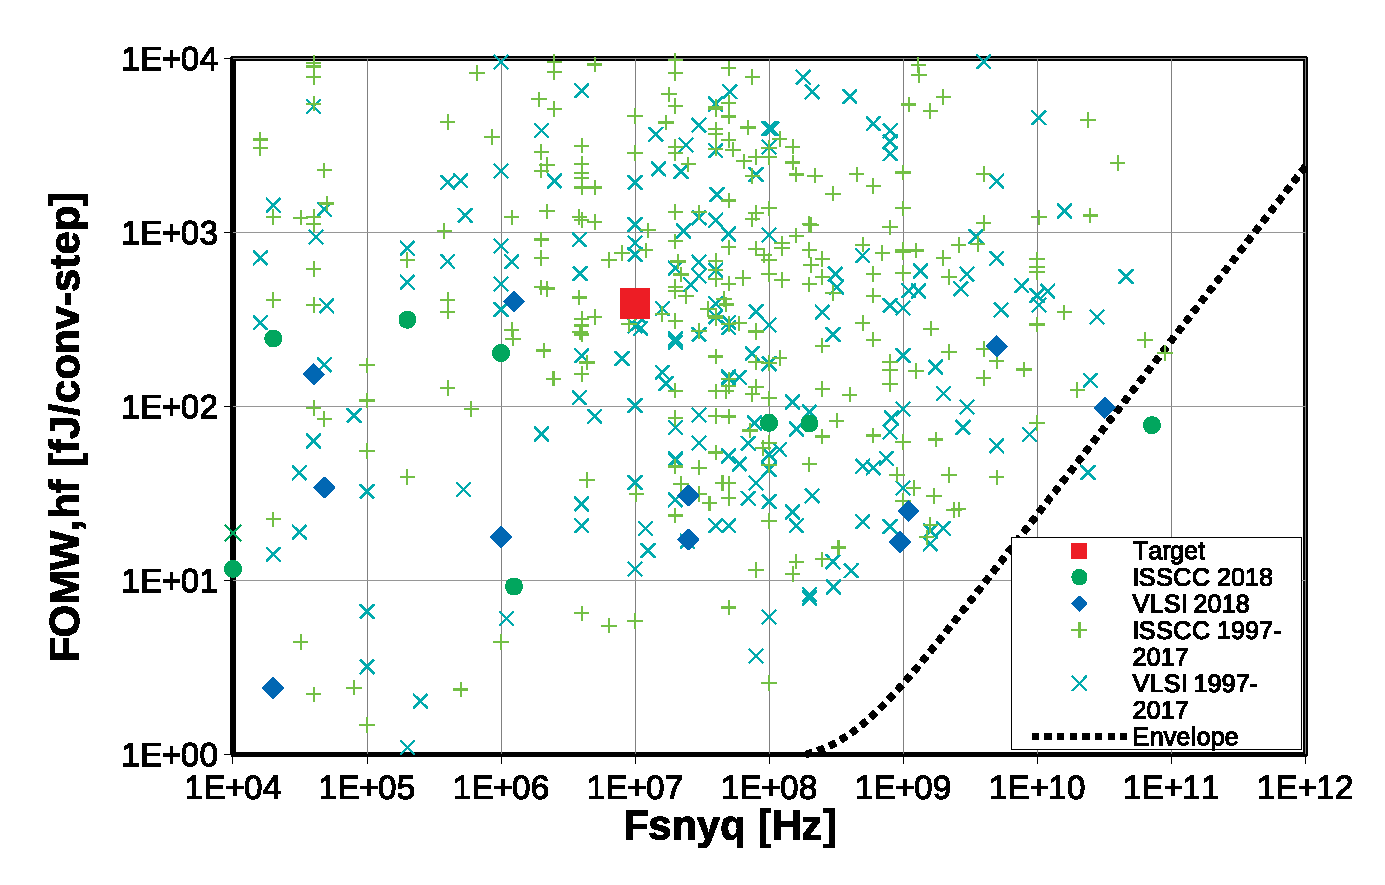
\includegraphics[width=.8\textwidth]{Chapter2/Figs/Vector/walden-fom-2018.eps}
    \caption{Walden FoM versus the nyquist frequency of ADC published in ISSCC and VLSI from 1997 to 2018 in comparison with the proposed one}
    \label{fig:walden-fom-comparison}
\end{figure}

This FoM is intended to provide a measure of how much energy is required to perform a conversion step, expressed in picojoules (pJ) per conversion step. This metric is created under the assumption that power tends to scale linearly with the input frequency and SNDR. However, In a high resolution ADC that is 10 bits or more, the resolution is mostly limited by thermal noise. Let us suppose the ADC is a capacitive load C, the noise is in the form of \(\sqrt{kT/C}\). In order to increase the resolution by 1 bit, C has to quadruple. If the operating frequency is kept constant, the power consumption has to be increased by a factor of four for an improvement of a factor of two in resolution. This implies that improving the resolution by 1 bit automatically worsens the FoM by a factor of two.

\figurename~\ref{fig:walden-fom-comparison} represents the Walden FoM from the Murmann ADC survey taking into account conferences until 2018. In addition the FoM of the proposed ADC is represented in the middle of these by a large bullet. With 15 mW at 20 Mhz it should be equal to 750 pJ with an SNDR = 68 dB. Even if the ADC is placed in the middle of the graph, the highest temperature of the operating range make the thermal noise the most limiting factor in our design challenging.

This figure of merit can also be represented in function of the surface per channel to represent the design effort to minimize the cost. Represented in \figurename~\ref{fig:walden-area-fom-comparison}, the ADC are concentrated along a line going from a low FoM with a small area (bottom left corner), to the high FoM with a large area (top right corner). The technology scaling down more and more ADC appear in the bottom left corner. The specification of the target ADC is right in the middle. Our primary goal is first to reduce the area, and then this FoM.

\begin{figure}[htp]
    \centering
    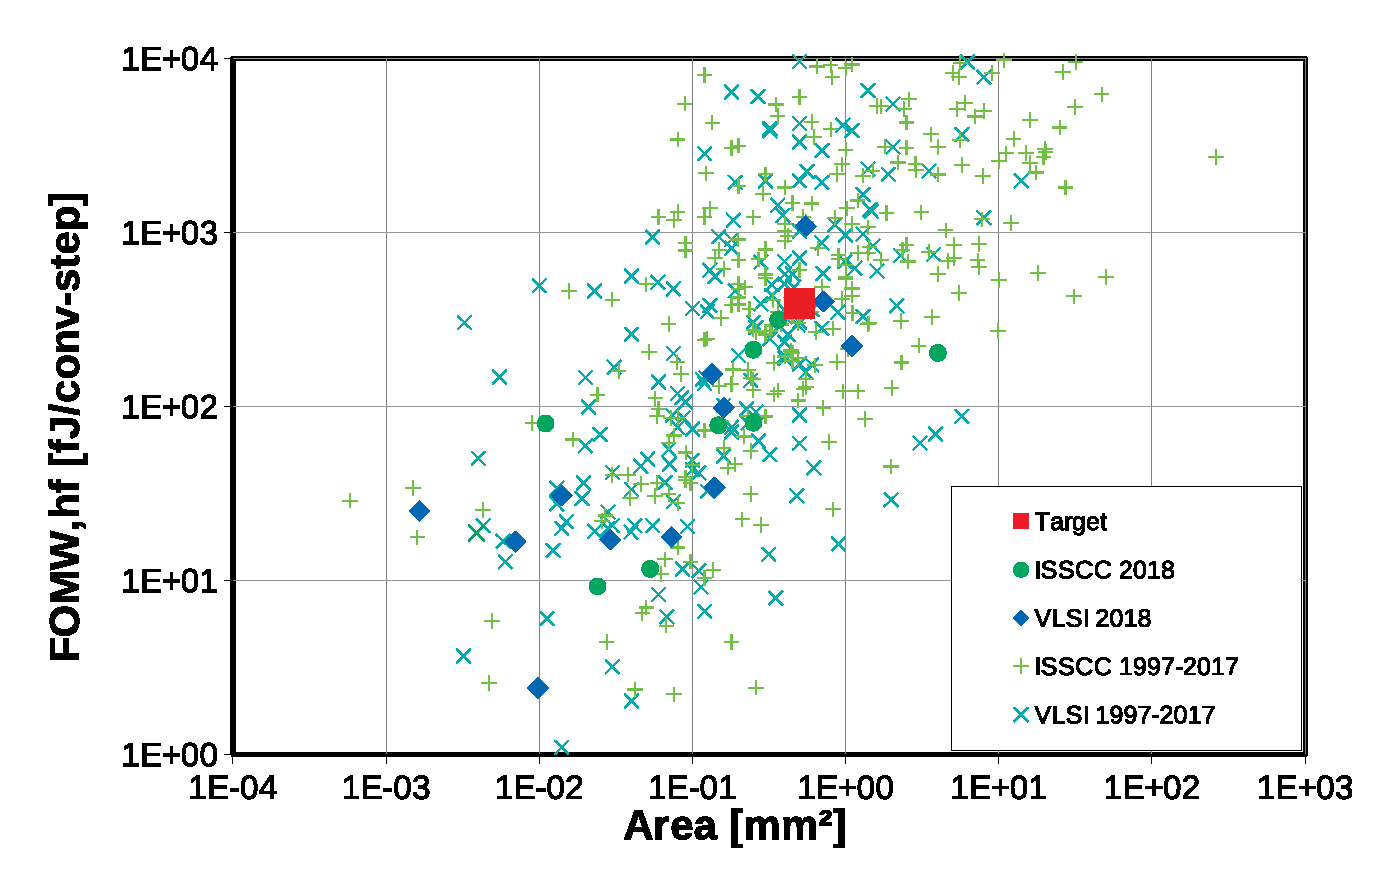
\includegraphics[width=.8\textwidth]{Chapter2/Figs/Vector/walden-fom-area-2018.eps}
    \caption{Walden FoM versus the area of ADC published in ISSCC and VLSI from 1997 to 2018 in comparison with the proposed one}
    \label{fig:walden-area-fom-comparison}
\end{figure}

\clearpage
